\documentclass[aspectratio=169]{beamer}
\usepackage{amsmath}
\usepackage{amssymb}
\usepackage{amsfonts}
\usepackage{graphicx}
\usepackage{luatexja} 
\usepackage{comment}
\usepackage{bm}
\usepackage{setspace}
\usepackage{caption}

\usetheme{LightTheme}
\setbeamertemplate{footline}[frame number]
\setbeamertemplate{navigation symbols}{}
%\setlength{\baselineskip}{10pt}
\begin{document}

% タイトルフレーム
\title{進捗状況}
\subtitle{TypescriptとReactコンポーネントの作成} 
\author{\small B4 小林紹子} % 必要に応じて変更・削除
\date{\small\today} % 必要に応じて変更・削除

\begin{frame}
    \titlepage
\end{frame}

\begin{frame}{目次}
    \tableofcontents
\end{frame}



\section{Typescript}

\begin{frame}{Typescript}
    \begin{itemize}
        \setlength{\itemsep}{1.5em} 
        \item \textbf{Typescriptのメリット}\\
        \begin{itemize}
            \setlength{\itemsep}{1.5em} 
            \item TypescriptはJavascriptを拡張している上方互換言語.
            \item 以下の機能を追加している.
            \begin{itemize}
                \item 型定義
                \item インタフェースとクラス
                \item null/undefined安全など
            \end{itemize}
        \end{itemize}
        \item \textbf{Typescriptのデメリット}
        \begin{itemize}
            \item 規模によってコンパイルに時間がかかる.
        \end{itemize}
    \end{itemize}
\end{frame}

\begin{frame}{Typescriptの自作サンプル一覧}
    \vspace{-1em}
    \begin{figure}
        \centering
        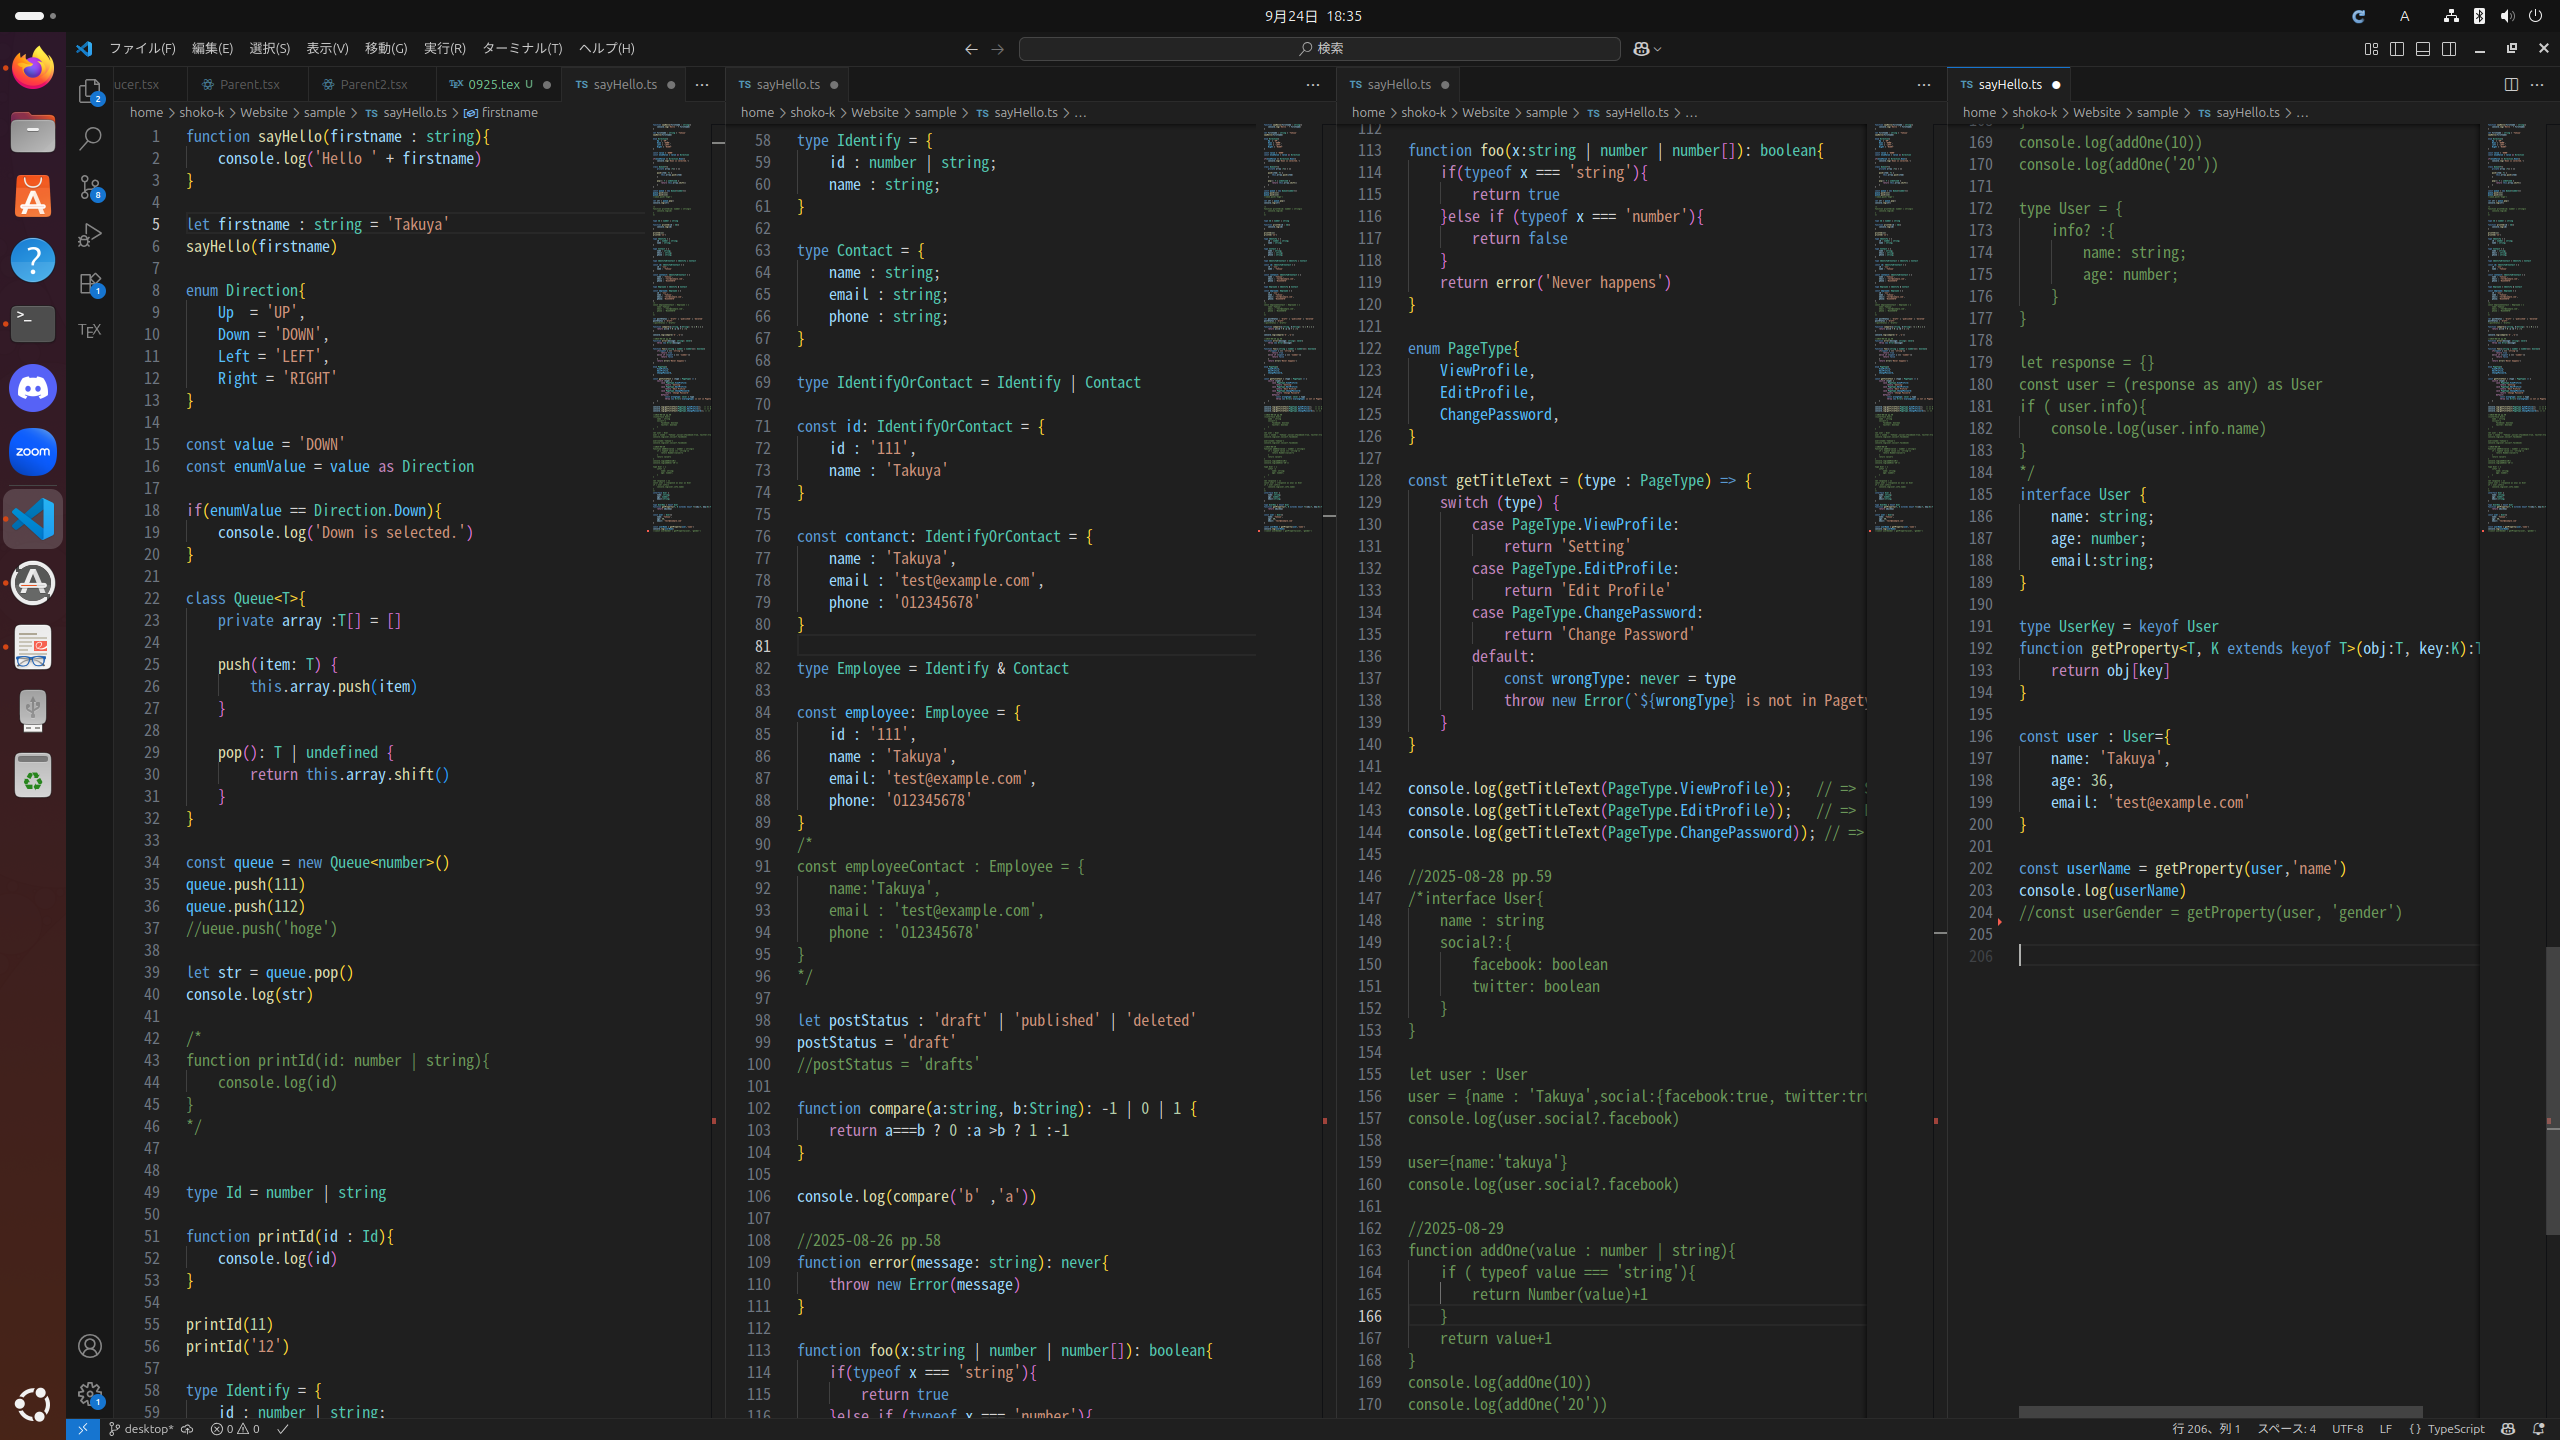
\includegraphics[width=\textwidth,height=\paperheight]{typescript_code.png}
    \end{figure}
\end{frame}

\section{React入門}

\begin{frame}{Reactの構成}
    Reactのプロジェクトは以下のようになっており,最終的には結合・最小化されたHTML/CSS/Javascriptのコードとなって出力される.
    \begin{figure}
        \centering
        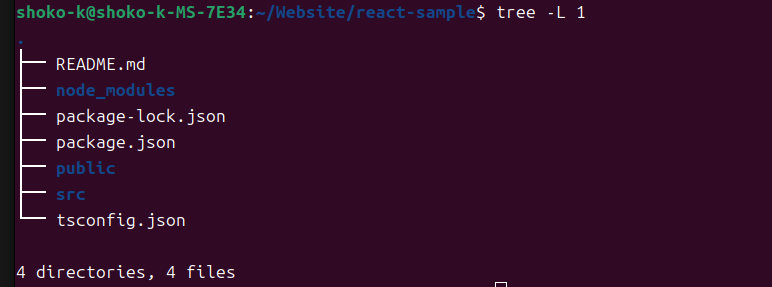
\includegraphics[scale = 0.3]{React_tree.png}
    \end{figure}
\end{frame}  

\begin{frame}{index.tsxをビルドしたJavaScriptが実行される}
    index.tsxには,JSXタグを用いてHTMLタグやコンポーネントを扱う.
    \begin{figure}
        \centering
        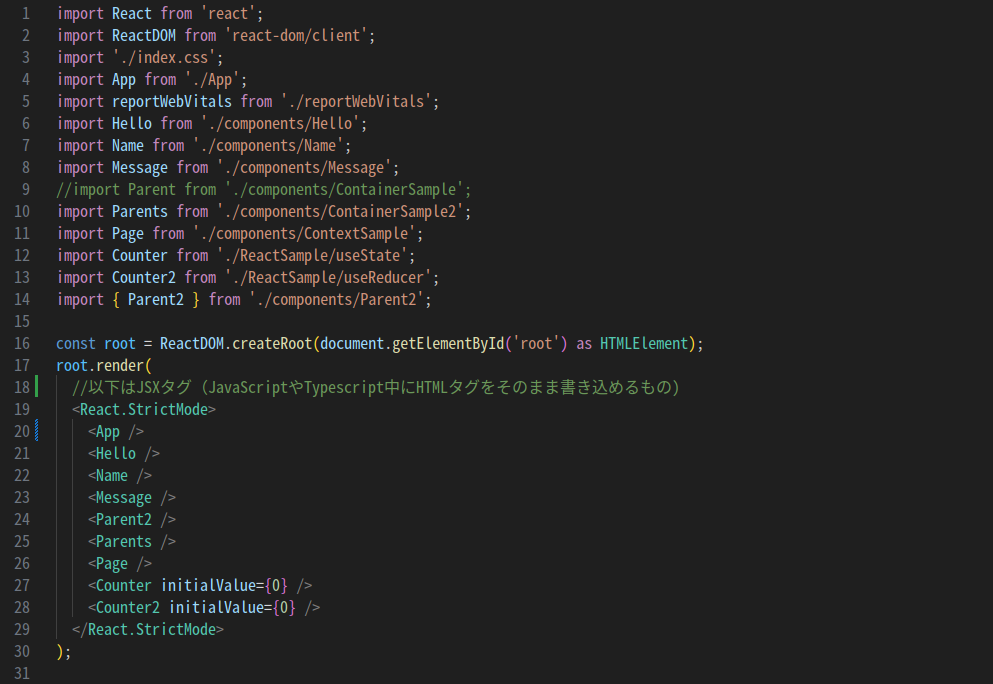
\includegraphics[scale = 0.25]{index_tsx.png}
    \end{figure}
\end{frame}  

\begin{frame}{App.tsx}
    それぞれの<App/>などはApp.tsxなどからインポートする.\\
    App.tsxでApp関数を作成し,JSXタグを用いてHTML要素を返す.
    \begin{figure}
        \centering
       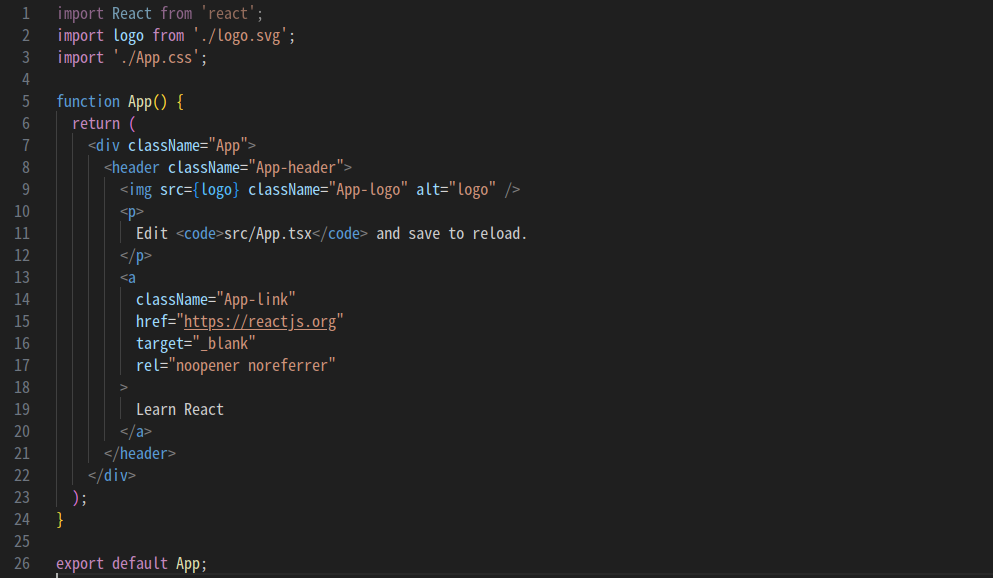
\includegraphics[scale = 0.3]{App_tsx.png}
    \end{figure}
\end{frame}  

\begin{frame}[allowframebreaks]{Webページができるまでの大まかな流れ}
    \begin{enumerate}
        \item public/index.htmlが読み込まれて,ブラウザに描画される.
        \item ブラウザがJavaScriptのコードを取得し,Reactを使ったコードの実行を開始する.
        \item render\(\)で与えられたAppをrootオブジェクト作成時に与えられたrootというIDを持つ要素以下に描画する.
    \end{enumerate}
    \begin{figure}
        \centering
       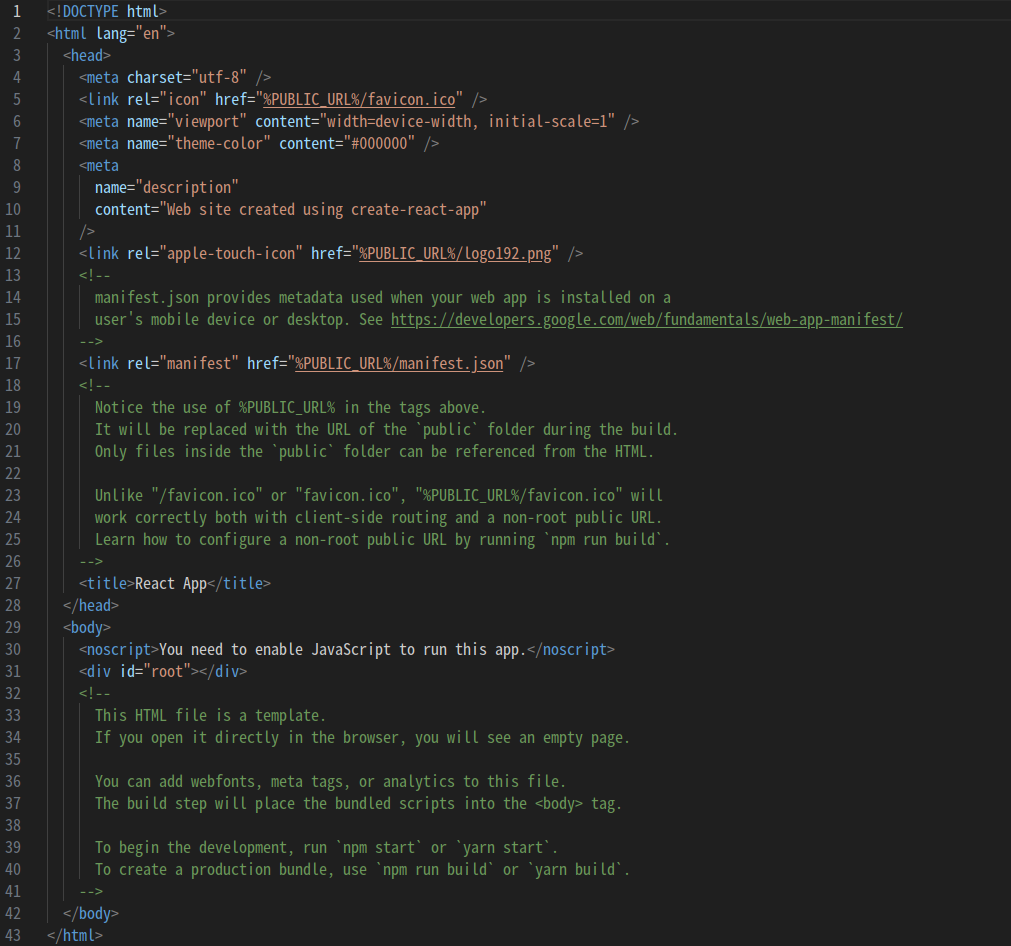
\includegraphics[height=\paperheight]{index_html.png}
    \end{figure}
\end{frame}

\section{Reactコンポーネントの作成}
\begin{frame}{Reactコンポーネントとは}
    \begin{itemize}
        \item 画面にどういう要素を表示するかを定義する設計図.
        \item 表示要素とその要素の挙動をセットにした部品.
        \item 何度も再利用できる部品のようなもの.
    \end{itemize}
    \begin{figure}
        \centering
       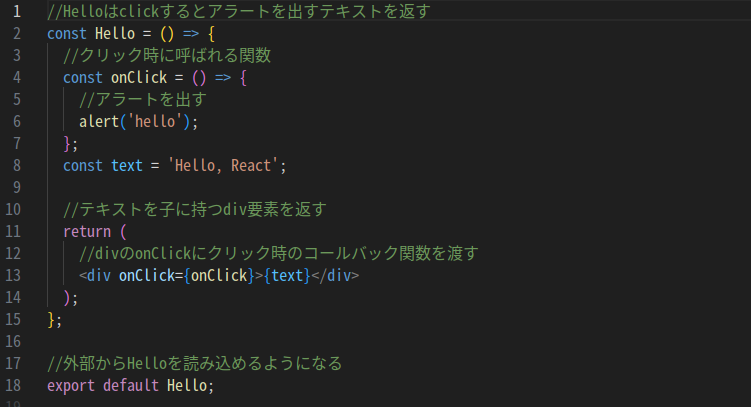
\includegraphics[scale=0.35]{Hello_tsx.png}
       \caption{例:Hello.tsx}
    \end{figure}
\end{frame}

\begin{frame}{テキスト入力}
    名前を入力するテキストボックスの作成.
    \begin{figure}
        \centering
       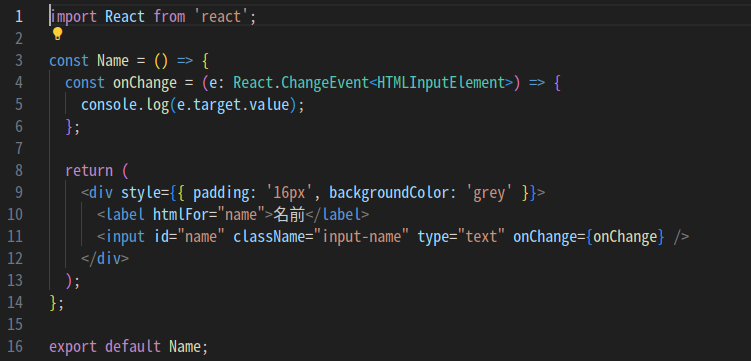
\includegraphics[scale=0.35]{Name_tsx.png}
       \caption{Name.tsx}
    \end{figure}
\end{frame}

\begin{frame}{コンポーネントの組み合わせ}
    Textコンポーネントを利用して,messageコンポーネントを作成する.
    \begin{figure}
        \centering
       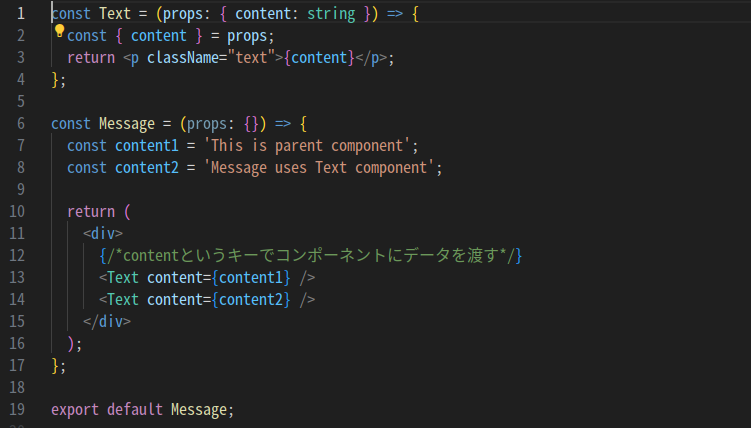
\includegraphics[scale=0.35]{Message_tsx.png}
       \caption{Message.tsx}
    \end{figure}
\end{frame}

\begin{frame}[allowframebreaks]{もっと自由な引数にする}
    React.ReactElementで<p>ここの部分が背景色で囲まれます</p>が読み込まれる.
    \begin{figure}
        \centering
       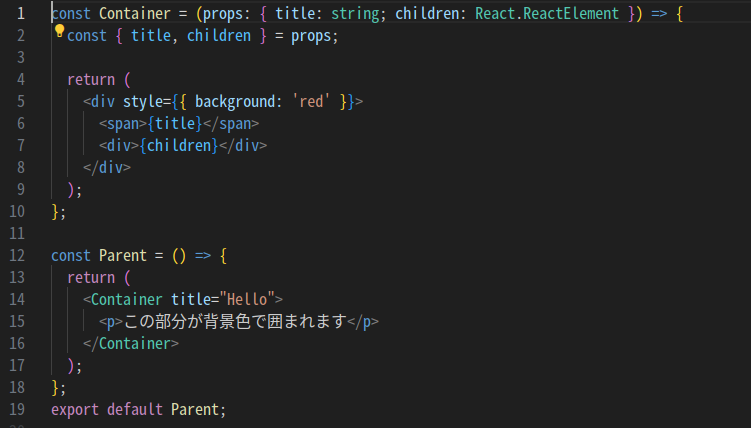
\includegraphics[scale=0.35]{ContainerSample_tsx.png}
       \caption{ContainerSample.tsx}
    \end{figure}
    \begin{figure}
        \centering
       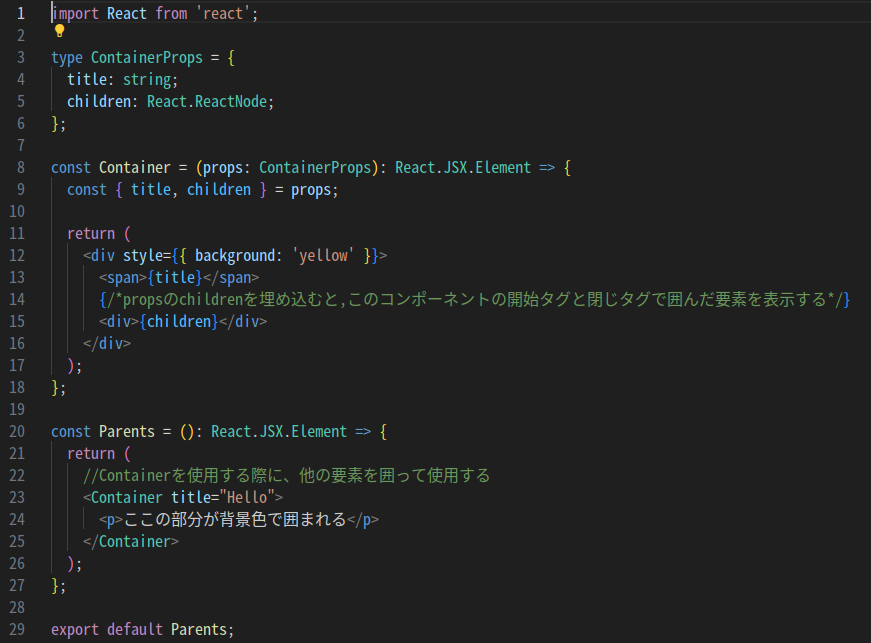
\includegraphics[scale=0.26]{ContainerSample2_tsx.png}
       \caption{ContainerSample2.tsx}
    \end{figure}
\end{frame}

\begin{frame}[allowframebreaks]{遠いところからもデータを受け取れるようにする}
    \begin{itemize}
        \item props:親から子へ任意のデータを渡す.
        \item Context:親以外からも必要なデータを参照する.
    \end{itemize}
    \begin{figure}
        \centering
       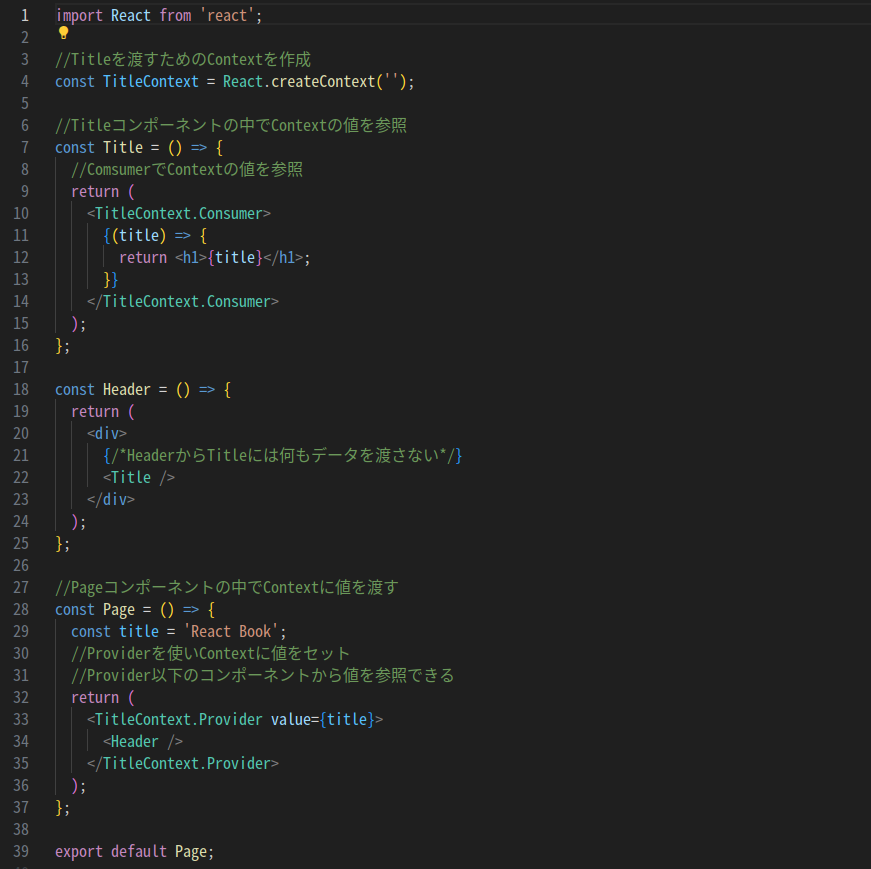
\includegraphics[scale=0.25]{ContextSample_tsx.png}
    \end{figure}
\end{frame}

\section{React\ Hook}
\begin{frame}{React\ Hook}
    \begin{itemize}
        \item React\ Hook:状態管理などクラスを書かずに使えるようになる機能.
        \item 全部で15種類ある.
        \item コンポーネントのコードを綺麗に保ち,コードの再利用性を高める.
    \end{itemize}
\end{frame}
\subsection{状態のフック}
\begin{frame}{useState}
    const[状態,更新関数]=useState(初期状態)\\
    更新関数を呼び出すと状態が変化し,コンポーネントが再描画される.\\
    \begin{figure}
        \centering
       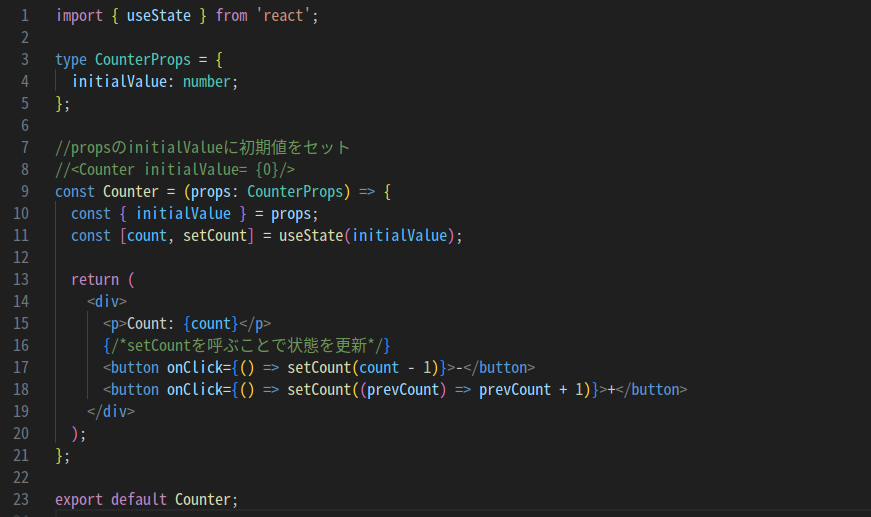
\includegraphics[scale=0.3]{useState.png}
       \caption{カウンター}
    \end{figure}
\end{frame}

\begin{frame}[allowframebreaks]{useReducer}
    useStateよりも多くの複雑な状態遷移を扱える\\
    現在の状態とactionを渡すと次の状態を返すreducerという関数を用いる.\\
    ボタンが押されるとdispatch関数を使ってactionを発出する.\\
    \begin{figure}
        \centering
       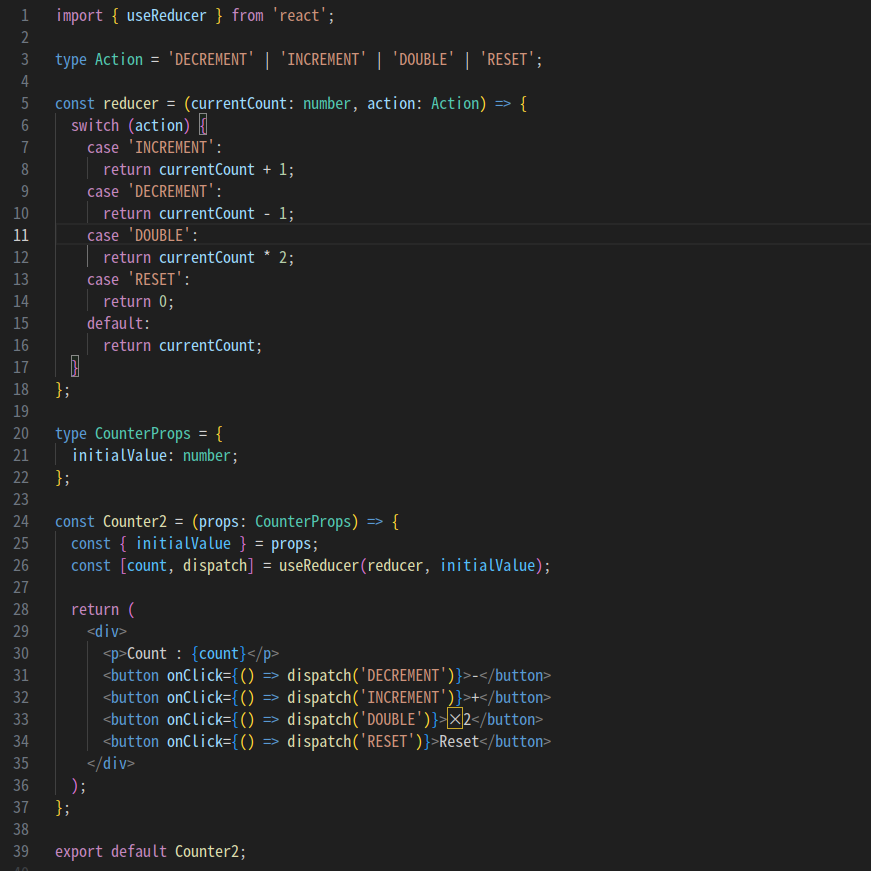
\includegraphics[scale=0.25]{useReducer.png}
       
    \end{figure}
\end{frame}

\subsection{メモ化のフック}
\begin{frame}[allowframebreaks]{メモ化コンポーネント}
    親コンポーネントが再描画されると子コンポーネントも自動的に描画される.\\
    この再描画の伝搬を止めるのに利用される.\\
    今回はmemo関数を用いている.
    \begin{figure}
        \centering
       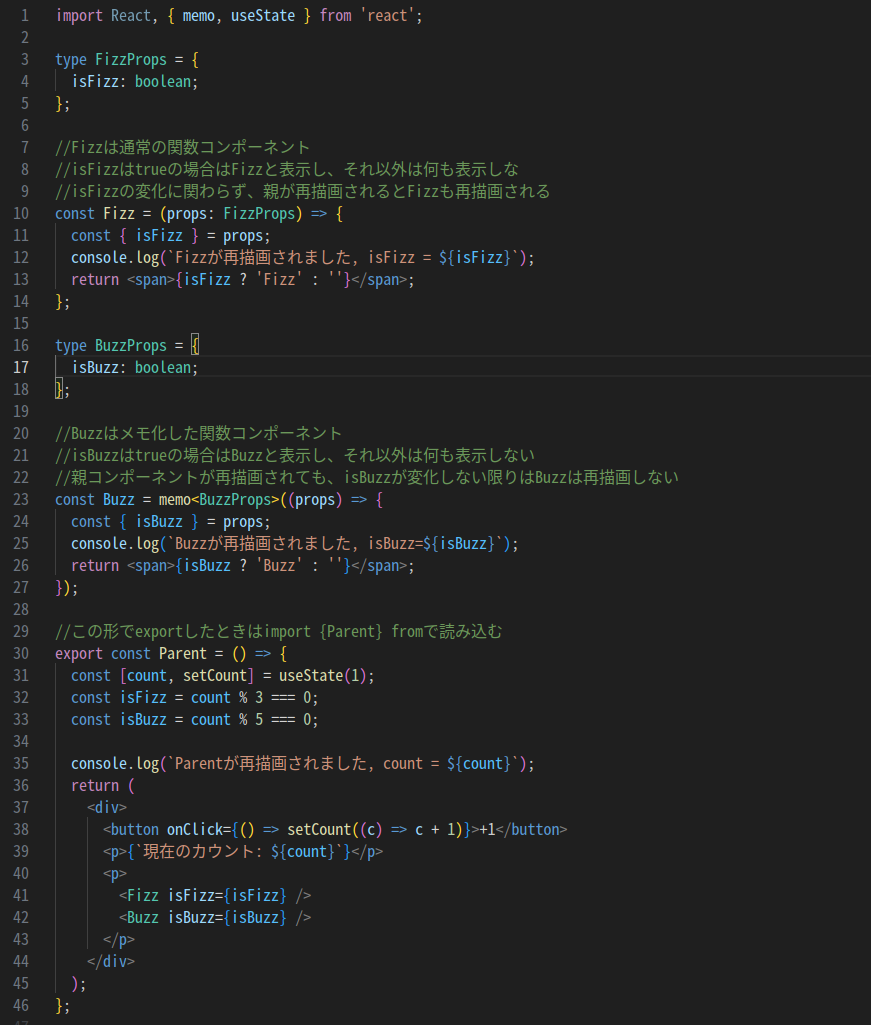
\includegraphics[scale=0.2]{Parent.png}
    \end{figure}
\end{frame}
\begin{frame}
    \begin{figure}
        \centering
       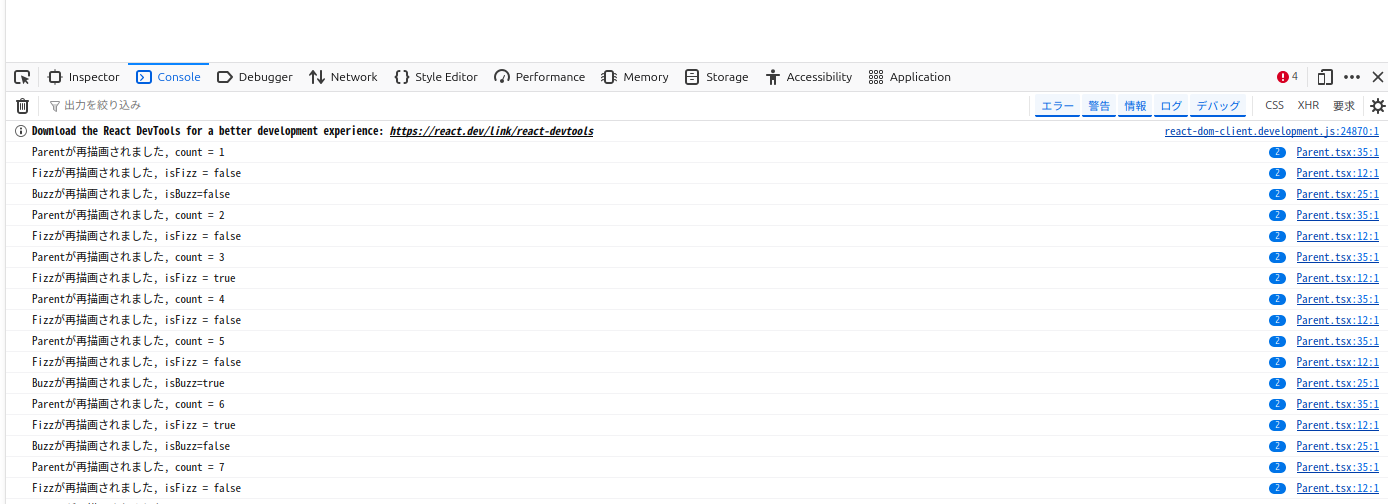
\includegraphics[scale=0.5]{result_Parent.png}
    \end{figure}
    
\end{frame}

\end{document}


